\documentclass[10pt, conference]{format/ieeeconf}

\IEEEoverridecommandlockouts    % Needed for \thanks command
\overrideIEEEmargins            % Needed to meet printer requirements.

\usepackage{glossaries}
\newacronym{ism}{ISM}{Inverse Sensor Model}
\newacronym{uav}{UAV}{Unmanned Aerial Vehicle}
\newacronym{fov}{FOV}{Field of View}


\bibliographystyle{format/IEEEtran}

% Tables
\usepackage{tabularx}
\usepackage{multirow, multicol}
\usepackage{array}
\newcolumntype{P}[1]{>{\centering\arraybackslash}p{#1}}
\newcolumntype{M}[1]{>{\centering\arraybackslash}m{#1}}
\usepackage{booktabs}
\newcolumntype{N}{>{\centering\arraybackslash}m{.5in}}
\newcolumntype{G}{>{\centering\arraybackslash}m{2in}}

% Comments
\newcommand\todo[1]{\textcolor{red}{#1}}
\newcommand\edited[1]{\textcolor{black}{#1}}
\newcommand\canremove[1]{\textcolor{blue}{#1}}

% XXX: Fix ieeeconf BS:
\let\labelindent\relax
\let\proof\relax
\let\endproof\relax

%====================================================================
%%XXX: Packages
%\usepackage[normalem]{ulem}	                        % underlining!
\usepackage[table,usenames,dvipsnames]{xcolor}      % color
\usepackage{extarrows}                              % http://ctan.org/pkg/extarrows
\usepackage{enumitem}
\usepackage{wrapfig}

%\usepackage[margins]{trackchanges}

% Math
\usepackage{amsmath,amssymb,amsfonts,amsthm,dsfont, bm} % math
\usepackage{mathtools}
\usepackage{algorithm,algorithmicx,listings}        % algorithms
\usepackage[noend]{algpseudocode}			              % necessary for algorithmicx
\makeatletter
\def\BState{\State\hskip-\ALG@thistlm}
\makeatother
\DeclarePairedDelimiter\abs{\lvert}{\rvert}%
\DeclarePairedDelimiter\norm{\lVert}{\rVert}%
% Swap the definition of \abs* and \norm*, so that \abs
% and \norm resizes the size of the brackets, and the 
% starred version does not.
\makeatletter
\let\oldabs\abs
\def\abs{\@ifstar{\oldabs}{\oldabs*}}
%
\let\oldnorm\norm
\def\norm{\@ifstar{\oldnorm}{\oldnorm*}}
\makeatother

% Figures
\usepackage{graphicx}
\usepackage{subcaption}
\usepackage{textcomp}
\usepackage[font=footnotesize]{caption}
\usepackage{subcaption}
\usepackage[breaklinks=true, colorlinks, bookmarks=true, citecolor=Black, urlcolor=Violet,linkcolor=Black]{hyperref}

%====================================================================
%%XXX: Commands
\def\liminf{\mathop{\lim\inf}\limits}	% EXAMPLE: \liminf_n A_n
\def\limsup{\mathop{\lim\sup}\limits}	%
\def\argmin{\mathop{\arg\min}\limits}	%
\def\argmax{\mathop{\arg\max}\limits}	%
% Write above and below equal sign
\newcommand{\longeq}[2]{\xlongequal[\!#2\!]{\!#1\!}}
% #1 = top; #2 = bottom; #3 = inequality (<,>,\leq,\geq)
\newcommand{\longineq}[3]{\overset{#1}{\underset{#2}{#3}}}
\newcommand{\indicator}{\mathds{1}}
\DeclareMathOperator{\tr}{tr}
\DeclareMathOperator{\per}{\mathbf{per}}
\def\deg{^{\circ}}
\def\negquad{\mkern-18mu}             % negative quad space
\def\negqquad{\mkern-36mu}            % negative qquad space
\newcommand{\txbx}[1]{\boxed{\text{#1}}}

\setlength{\marginparwidth}{1.5cm}



\usepackage[normalem]{ulem}
\usepackage[utf8]{inputenc}
\usepackage[english]{babel}
\usepackage{hyperref}
\hypersetup{
    colorlinks=true,
    linkcolor=blue,
    filecolor=magenta,      
    urlcolor=cyan,
}

\newcommand{\prl}[1]{\mathopen{}\left(#1\right)\mathclose{}}
\newcommand{\brl}[1]{\mathopen{}\left[#1\right]\mathclose{}}
\newcommand{\crl}[1]{\mathopen{}\left\{#1\right\}\mathclose{}}
% MATH HELPER FUNCTIONS
\def\argmin{\mathop{\arg\min}\limits}	%
\def\argmax{\mathop{\arg\max}\limits}	%
\newcommand{\mat}[1]{\boldsymbol{\mathbf{#1}}}


\DeclareMathAlphabet\mathbfcal{OMS}{cmsy}{b}{n}

\usepackage[space, compress, sort]{cite}
\newtheorem{theorem}{Theorem}
\newtheorem{proposition}{Proposition}
\newtheorem{corollary}{Corollary}
\newtheorem{definition}{Definition}
\newtheorem{assumption}{Assumption}
\newtheorem*{assumption*}{Assumption}
\newtheorem{remark}{Remark}
\newtheorem*{problem*}{Problem}
\newtheorem{problem}{Problem}
\newtheorem{lemma}{Lemma}

\usepackage{lipsum}
\usepackage[capitalise]{cleveref}

\begin{document}

% \title{Behavior Guided Indoor MAV Exploration with Learned Information Prediction}
\title{Sensor Fusion of Depth Camera and Ultrasonic Sensor for Glass Detection}
% Capitalization of the title

% Make room for more info lines in the \author command  
\author{Beiming Li}
% Paper headers 
\maketitle

\begin{abstract}
We investigate the challenge posed by glass windows, which are common components in indoor environments, as they are not detectable by depth cameras. In contrast, ultrasonic sensors emit high-pitched sound pulses that are reflected regardless of lighting conditions or object's optical properties. Therefore, we investigate the feasibility of integrating ultrasonic sensors as a secondary sensing modality to our current mapping stack. The outcomes of this independent study include the development of simulation environments in Gazebo to replicate indoor building with windows, the implementation of a sensor fusion mechanism for combining depth image and sonar data, and the design of a RANSAC-based approach for window segmentation in indoor exploration scenarios. These outcomes enable the robot to recognize glass as obstacles and identify potential window regions based on geometric characteristics. This study provides insights into potential benefits and limitations of sensor fusion of depth camera and ultrasonic sensor.

\end{abstract}
    \section{Introduction}
\label{sec:intro}

Depth cameras have been popular in the field of robotics due to their ability to provide detailed environmental information that is useful for localization and mapping tasks, all while being cost-effective. However, these cameras are limited by two inherent drawbacks. Firstly, their sensing accuracy is significantly reduced when exposed to direct sunlight. Secondly, they are unable to detect transparent glass walls, which is also a limitation for LiDAR and Radar. On the other hand, ultrasonic sensors emit high-pitched sound pulses that are reflected regardless of lighting conditions or object's optical properties.

Therefore, we propose investigating the feasibility of integrating ultrasonic sensors as a secondary sensing modality to our current mapping stack. The benefits of combining ultrasonic sensors are manifold. Firstly, they are lightweight and cost-effective, making them suitable for widespread deployment on \glspl{uav} without increasing payload significantly. Additionally, they provide safety guarantees in environments that may contain glass walls or direct sunlight exposure, which is especially important for \gls{uav} navigation.

However, ultrasonic sensors suffer from low resolutions due to the multi-echo effect of sound waves, as well as lower sensing frequency compared to optical-based sensors. Furthermore, unlike depth cameras and radar arrays that provide image-like sensing feedback, ultrasonic sensors only provide one data point for each time-step, which is the measured distance to the nearest object in its field of view. Given the greater accuracy and detail provided by depth cameras, we use ToF cameras as the primary sensing device, while considering ultrasonic data as heuristic information. 

In summary, outcomes of this independent study are:
\begin{itemize}
    \item Developed simulation environments in Gazebo to replicate indoor building with windows and added customized sonar model to the existing drone model.
    \item Implemented sensor fusion mechanism for combining depth image and sonar data when maintaining an occupancy map, enabling the robot to recognize glass as obstacles. Used an inverse sensor model and sonar beam discretization during the occupancy probability update.
    \item Designed a RANSAC-based approach for window segmentation in indoor exploration scenarios, which identifies potential window regions based on sonar readings, depth-camera-based occupancy map and geometric characteristics.
\end{itemize}







    
    \section{Related Work}
\label{sec:related work}

% Exploration Strategy: Frontier based, Information based (sampling based), Mixed(hierarchical) approach
% Map Prediction: database, deep learning

\subsection{Ultrasonic Sensor Model}
The literature contains various models for ultrasonic sensors that are used in robot mapping and navigation applications. For example, in \cite{mapping2017} and \cite{advanced_sonar_sensor}, sonars are modeled as a 2D circular sector, where the sector angle and radius are determined by the sensing range of the hardware. On the other hand, \cite{multiray} proposes a model where the sonar beam is discretized into multiple rays, originating from the sensor center. This approach allows for a reduction in computational complexity and a more accurate representation of the irregular polygon shape of the sonar beam.

Given the beam pattern of the actual sensor attached to our UAV platform, we determined that it was unnecessary to adapt the multiple-ray discretization approach. However, since we also required the ability to perform 3D mapping, we modeled the sonar beam as a spherical cone. This approach extends the 2D circular sector model to its 3D counterpart and provides us with the necessary data to update and maintain a 3D occupancy map using sonar readings.

To accomplish this, we implemented an \gls{ism}, which encodes the probability that a given location in the environment contains an object. We extended the 2D \gls{ism} proposed in \cite{advanced_sonar_sensor} and \cite{wideanglesonar} to 3D to update and maintain a 3D occupancy map with sonar readings. Further details on our approach will be discussed in section \ref{sec:method_model}.

\subsection{Sensor Fusion with Ultrasonic Sensor}
Multiple studies have been conducted to integrate the ultrasonic sensor with either a camera or a LiDAR for robot mapping and navigation purposes. One such work is presented in \cite{lidarfusion}, where a fusion approach combining the ultrasonic sensor with a 2D LiDAR is proposed. Their method involves maintaining a single occupancy map, wherein the probability of each grid being occupied is updated at each time step by fusing sensor outputs. Notably, various sensor fusion algorithms, including the Linear Opinion Pool and the classic Bayes Filter, are evaluated to determine their effectiveness.

In addition to LiDAR, combining ultrasonic sensors with cameras has been investigated by several studies such as \cite{camerafusion} and \cite{obsavoid}. Of these, \cite{camerafusion} is particularly relevant to our task, as it has demonstrated the ability to detect moderate-sized glass walls. Unlike \cite{lidarfusion}, \cite{camerafusion} maintains two separate maps for depth camera and sonar data. The sonar map is updated only when the sonar reading provides information not present in the camera-based map. Finally, the two maps are merged into a single occupancy map. 

\subsection{Glass Segmentation}
The works discussed above have successfully addressed the issue of detecting glass as obstacles to enhance the safety of robot navigation. However, none of these works can provide segmentation information, i.e., the ability to distinguish glass from other semantic objects. Many existing studies have tackled the problem of glass segmentation using learning-based methods that take a single RGB or RGB-D image as input and generate a semantic mask for the glass region as output, as discussed in \cite{depthaware} and \cite{donthit}. However, such methods may prove to be computationally burdensome for UAV platforms, which are already limited in computational power and may not be able to support another large network solely for glass segmentation. Instead of learning-based methods, we propose a RANSAC-based segmentation approach. In indoor scenarios, most glass is typically windows framed by walls. Given a depth-camera-based occupancy map, RANSAC could detect the largest plane, which should correspond to straight walls in an indoor setting. We could then locate potential window regions based on geometric information. Further details on this approach will be provided in Section \ref{sec:method_ransac}.
    
    \section{Method and Results}
\label{sec:method}

\subsection{Simulation Environment}
\label{sec:method_sim}

We developed a collection of simulation environments in Gazebo, specifically designed to replicate the layouts of typical indoor building floor plans. In addition, we have augmented the existing dragon ddk drone model with a customized ultrasonic model, enabling the simulated drone to provide simulated sonar feedback.

An example of our simulation environments is presented in Fig. \ref{fig:sim_env}, depicting an indoor building with a single loop of hallway and multiple small rooms. Along the outer walls, there are a series of empty rectangle areas representing windows. We have set the collision properties of the window material to be identical to that of the wall material. This enables us to simulate scenarios where the drone may collide with windows during navigation. Furthermore, in order to replicate the behavior of real-world depth cameras, the windows are set to be invisible to the simulated depth camera module, which is accomplished by setting the visual properties of the window material to be empty, effectively rendering the window areas transparent in depth camera images captured by the simulated drone. 

\begin{figure}[h]
    \centering
    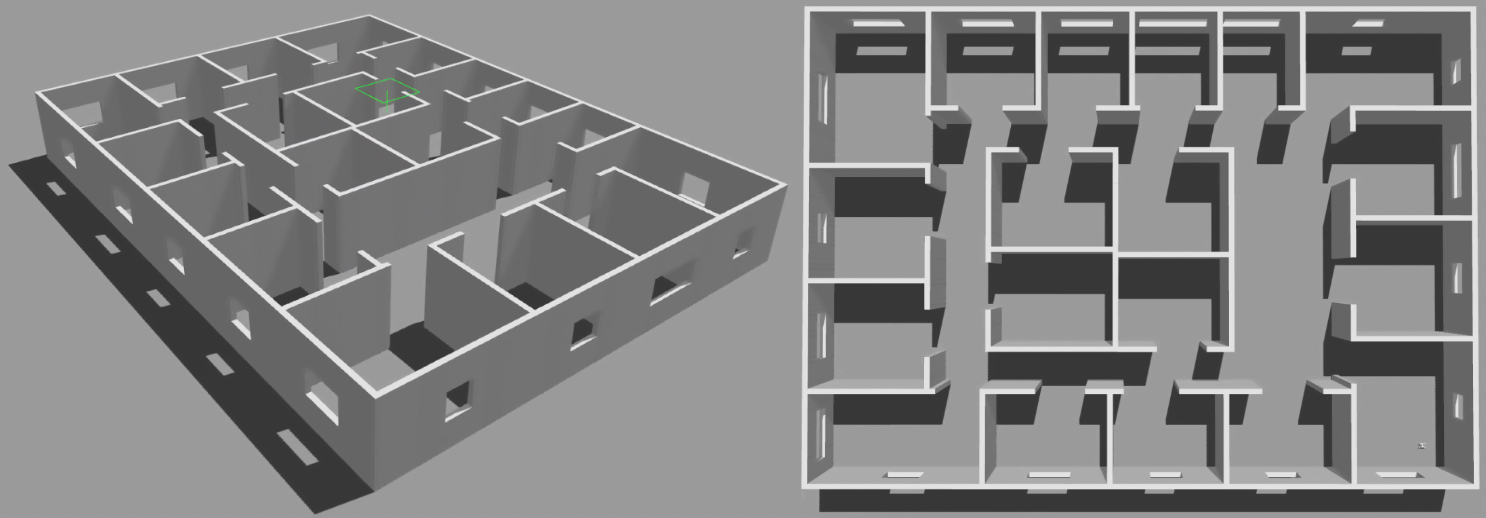
\includegraphics[width=1.0\columnwidth]{fig/sim_env.png}
    \caption{Example of simulation environments,}
    \label{fig:sim_env}
\end{figure}

Besides, we have integrated a customized sonar model into the description file of the dragon ddk drone model. Drawing upon the gazebo range sensor plugin, we have established a series of parameters to accurately reflect the specifications of our actual sonar hardware. This includes variables such as update rate, maximum sensor range, and \glspl{fov}. As the range sensor plugin detects obstacles based on collision properties of the material, we have designed the window material in such a way that it remains detectable to the sonar model. The resulting simulation enables us to replicate various real-world scenarios, such as the drone's encounter with a window, as depicted in the left figure. In this case, the occupancy map, maintained by the depth camera point clouds, does not mark the window area as an obstacle. However, the sonar sensor provides accurate distance measurements to the window, which is visualized as a dark cone originating from the drone.

\begin{figure}[h]
    \centering
    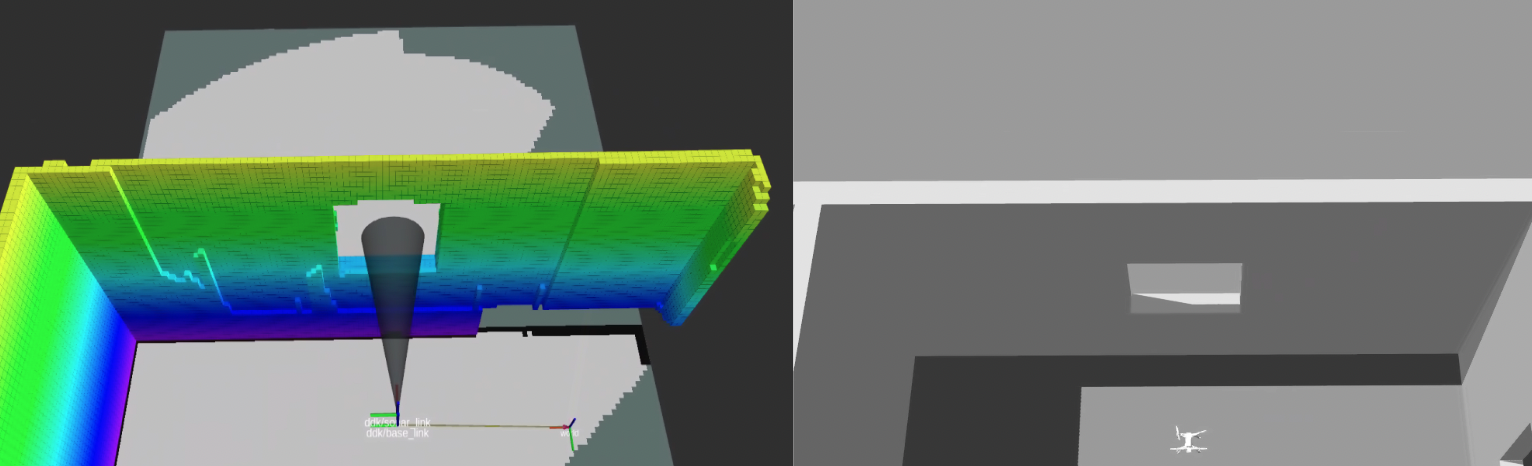
\includegraphics[width=1.0\columnwidth]{fig/sim_sonar.png}
    \caption{Simulated sonar feedback. The right figure shows the drone (white) is facing a wall with a small window in Gazebo simulation. The left figure shows the depth-camera-based occupancy map and the simulated sonar feedback (black cone).}
    \label{fig:sim_sonar}
\end{figure}

\subsection{Inverse Sensor Model}
\label{sec:method_model}
The adaptation of the 3D sonar sensor model stems from the 2D model proposed in \cite{wideanglesonar}. The model accounts for both empty and occupied regions, taking into consideration the range and direction of the grids within the sonar beam. Fig. \ref{fig:sim_sonar_2d}  from \cite{advanced_sonar_sensor} presents a clear representation of a 2D sector of a 3D sonar beam, where the X-axis denotes the direction towards which the sonar sensor is pointing (referred as sonar beam center). The figure corresponds to a sonar beam having a \gls{fov} of $\omega_i$ and a range measurement of $z_i$.

Given a point $p_i$ within the sonar beam and situated at a distance of $r_i$ meters away from the sonar sensor, connecting $p_i$ to the sonar results in a line that forms an angle of $\theta_i$ with the sonar beam center.

\begin{figure}[h]
    \centering
    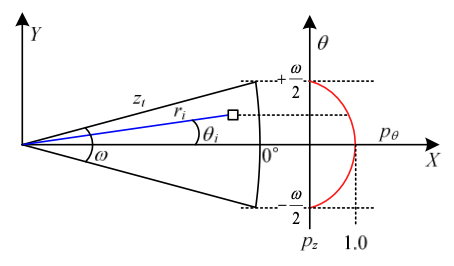
\includegraphics[width=0.5\columnwidth]{fig/sonar_model_2d.png}
    \caption{2D sector of a sonar beam}
    \label{fig:sim_sonar_2d}
\end{figure}

First, we derived a decay term based on $\theta_i$, which is distributed in a semicircular shape as shown in the right-hand side of Fig. \ref{fig:sim_sonar_2d}. The decay term $\alpha_i$ is formulated as:
\begin{equation}
    \alpha_{i} = 1 - (\frac{2 * \theta_i}{\omega})^2
\end{equation}

For a ray of angle $\theta_i$, we compute a decayed $p_{\text{hit}_i}^{\prime}$ and a decayed $p_{\text{miss}_i}^{\prime}$ as below, where $p_{\text{hit}}$ and $p_{\text{miss}}$ is a predefined constant (which is set to 0.7 and 0.3 respectively):
\begin{equation}
    \begin{split}
    p_{\text{hit}_i}^{\prime} = 0.5 + (p_{\text{hit}} - 0.5) * \alpha_{i} \\
    p_{\text{miss}_i}^{\prime} = 0.5 - (0.5 - p_{\text{miss}}) * \alpha_{i}
    \end{split}
\end{equation}

Finally, the occupancy probability of $p_i$ is formulated as follows, where $\epsilon$ is a predefined constant that reflects the expected accuracy of the sonar sensor (which is set to 0.05):
\begin{equation}
    p_{p_i} =
    \begin{cases}
      p_{\text{miss}_i}^{\prime} + (\frac{r_i}{z_i- \epsilon})^2(0.5 - p_{\text{miss}_i}^{\prime}) & \hspace{-3pt}\text{if $r_i \leq z_i- \epsilon$} \\
      p_{\text{hit}_i}^{\prime} - (\frac{r_i - z_i}{\epsilon})^2(p_{\text{hit}_i}^{\prime} - 0.5) & \hspace{-3pt}\text{if $|r_i - z_i| < \epsilon$}
    \end{cases}
\end{equation}

For a better grasp of the sonar model, we have presented a visualization of the occupancy probability along four rays that vary in angles with the sonar beam center in Fig. \ref{fig:sim_sonar_plot}.
\begin{figure}[h]
    \centering
    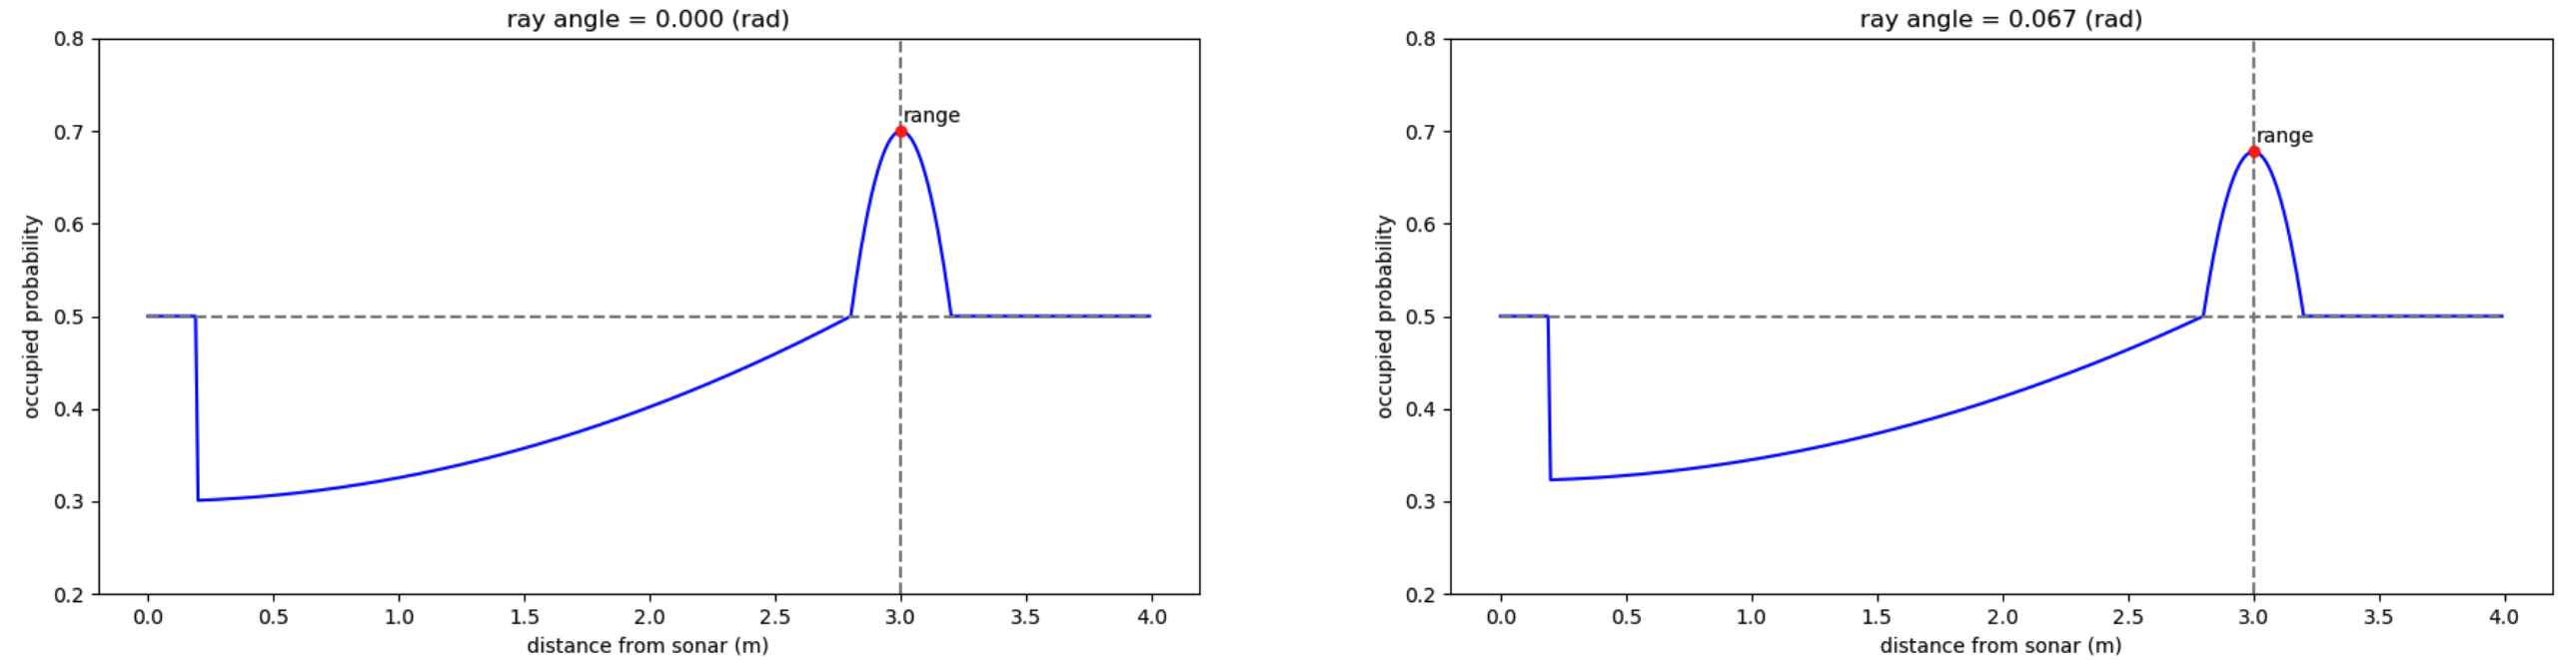
\includegraphics[width=1.0\columnwidth]{fig/sonar_model_1.png}
    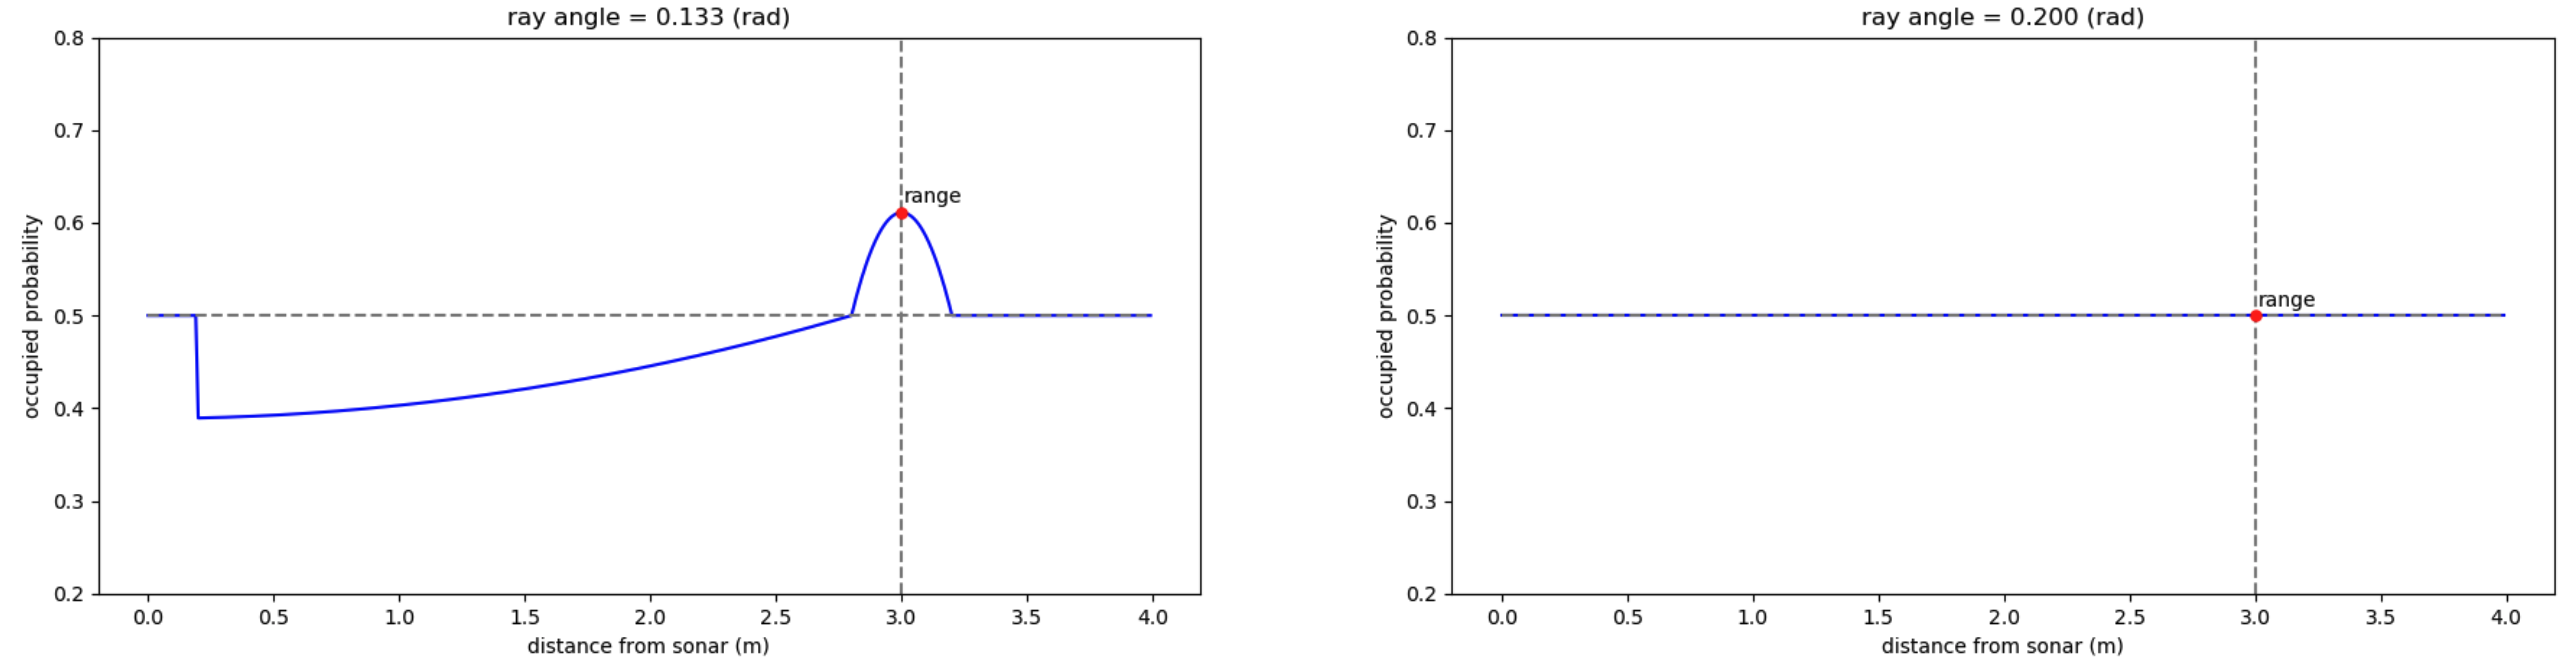
\includegraphics[width=1.0\columnwidth]{fig/sonar_model_2.png}
    \caption{Sonar Inverse Sensor Model Examples: occupancy probability along rays that have different angles with sonar beam center, notice that the sonar \gls{fov} is set the 0.4 rad.}
    \label{fig:sim_sonar_plot}
\end{figure}

As illustrated by Fig. \ref{fig:sim_sonar_plot}, we are more confident with the occupied condition along rays that have smaller angles with the sonar beam center, hence the occupancy probability is updated more confidently. Conversely, the occupied condition near the edge of the sonar beam is less certain, resulting in a more conservative update of the occupancy probability.

\subsection{Sonar Beam Discretization}
\label{sec:method_dis}
Unlike depth images, sonar readings are only scalar values. In order to update the probability of each relevant grid cell in the occupancy map, we need an effective way to discretize the sonar beam.

To address this, we chose to discretize the bottom surface of the spherical cone into dense equidistributed points. This enables us to use the classic ray tracing algorithm \cite{raytracing} to traverse all the grid cells that lie within the sonar beam.

To begin with, a point on the spherical surface can be represented using the classical spherical coordinates, in which a point is addressed via the polar angle $\theta$ and the azimuthal angle $\phi$. If the sphere has a radius $r$, the Cartesian coordinates of that point are given by:
\begin{equation}
    \label{eq:point}
    \begin{pmatrix}
    X \\ Y \\ Z
    \end{pmatrix} = 
    r 
    \begin{pmatrix}
    sin\theta cos\phi\\
    sin\theta sin\phi\\
    cos\phi
    \end{pmatrix}
\end{equation}

The discretization of the spherical cap of our interest is based on the approach proposed in \cite{equidist}, with modifications. In Algorithm~\ref{alg:equidist}, $N$ represents the desired number of points, and $\omega$ represents the \gls{fov} of the sonar sensor. To achieve a nearly regular equidistribution, we first choose circles of latitude at constant intervals $d_{\theta}$, and then on these circles, we choose points at constant intervals $d_{\phi}$. The selection of $d_{\theta}$ and $d_{\phi}$ is made to satisfy the condition $d_{\theta} \approx d_{\phi}$.

\begin{figure}[t]
\begin{algorithm}[H]
\scriptsize
\captionsetup{font=scriptsize} % set size of caption font
\caption{Generate equidistributed points on the spherical cap}\label{alg:equidist}
\begin{algorithmic} [1]
\State $a \gets$ $4\pi / N$;
\State $M_{\theta} \gets \lceil \pi / \sqrt{a} \rceil$;
\State $d_{\theta} \gets \pi / M_{\theta}$;
\State $d_{\phi} \gets a / d_{\theta}$;
\For{each $m$ in $0, ..., M_{\theta} - 1$}
\State $\theta \gets$ $\pi (m + 0.5) / M_{\theta}$;
\If{$\theta > \omega$ / 2}
    \State break;
\EndIf
\State $M_{\phi} \gets \lceil 2\pi sin\theta/ d_{\phi} \rceil$;
    \For{each $n$ in $0, ..., M_{\phi} - 1$}
        \State $\phi \gets$ $2\pi n / M_{\phi}$;
        \State create a point using Eq. \ref{eq:point}
    \EndFor
\EndFor
\end{algorithmic}
\end{algorithm}
\vspace{-1cm}
\end{figure}

\subsection{Occupancy Map Update}
\label{sec:method_occ}
To maintain an accurate and comprehensive representation of the surrounding environment, we maintained two separate occupancy maps. The first occupancy map is created solely using depth camera data, which provides reliable and precise information about the environment. The second occupancy map is updated with sonar readings, which can detect objects that are not visible to the camera.

To update the sonar occupancy map, we use the classic ray tracing algorithm, accompanied by the sonar's \gls{ism} and beam discretization method described in previous sections. However, not all sonar readings are accurate or informative, so we filter the readings based on their correspondence with the depth camera data. We consider three cases of sonar and depth camera correspondence. In case (a), the camera layer marks multiple cells inside the sonar beam as occupied, we assume that both sensors detected the same object, and we discard the sonar data. In case (b), the camera layer marks multiple cells inside the free space of the sonar beam as occupied, we assume that the sonar measurement is incorrect, and we discard the sonar data. In case (c), the camera does not detect anything, while the sonar receives reflections from objects within its sensing range, we suspect that there may be a glass wall in front of the robot. In this case, we update the sonar occupancy map with the current sonar reading.

\begin{figure}[h]
    \centering
    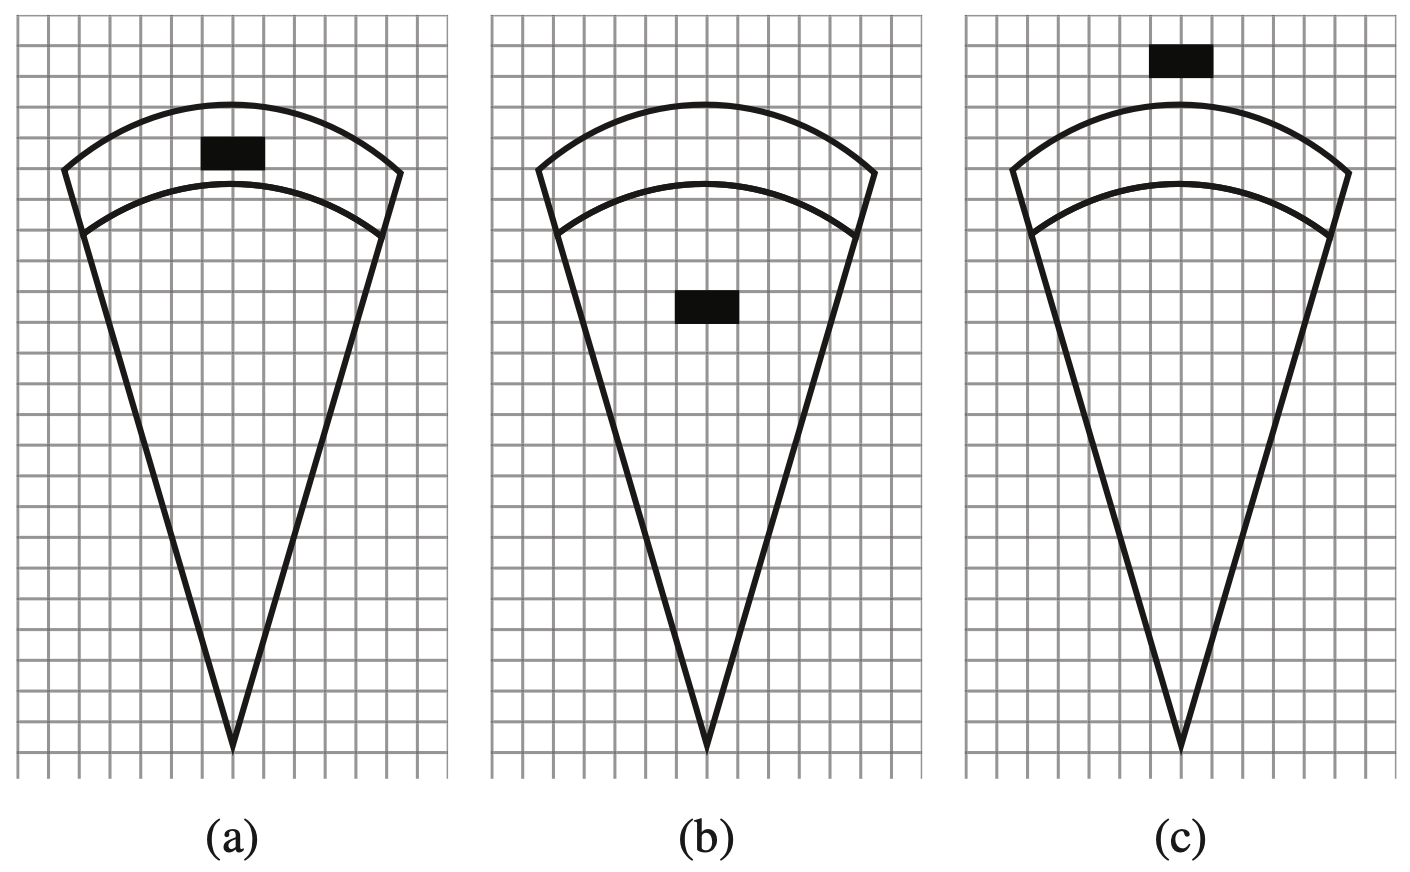
\includegraphics[width=0.8\columnwidth]{fig/occ.png}
    \caption{Three Cases of Sonar-Depth Correspondence.}
    \label{fig:occ}
\end{figure}

We illustrate these three cases in 2D space in Fig. \ref{fig:occ} from \cite{camerafusion}, where the underlying grid represents the current occupancy map created solely by the depth camera. Black cells represent objects, and white cells represent free space. The sonar beam is visualized and divided into two parts, with the lower part representing free space and the upper part representing the region where the sonar detects objects. The flow chart in Fig. \ref{fig:occ_flow} visualizes the mechanism described above.

\begin{figure}[h]
    \centering
    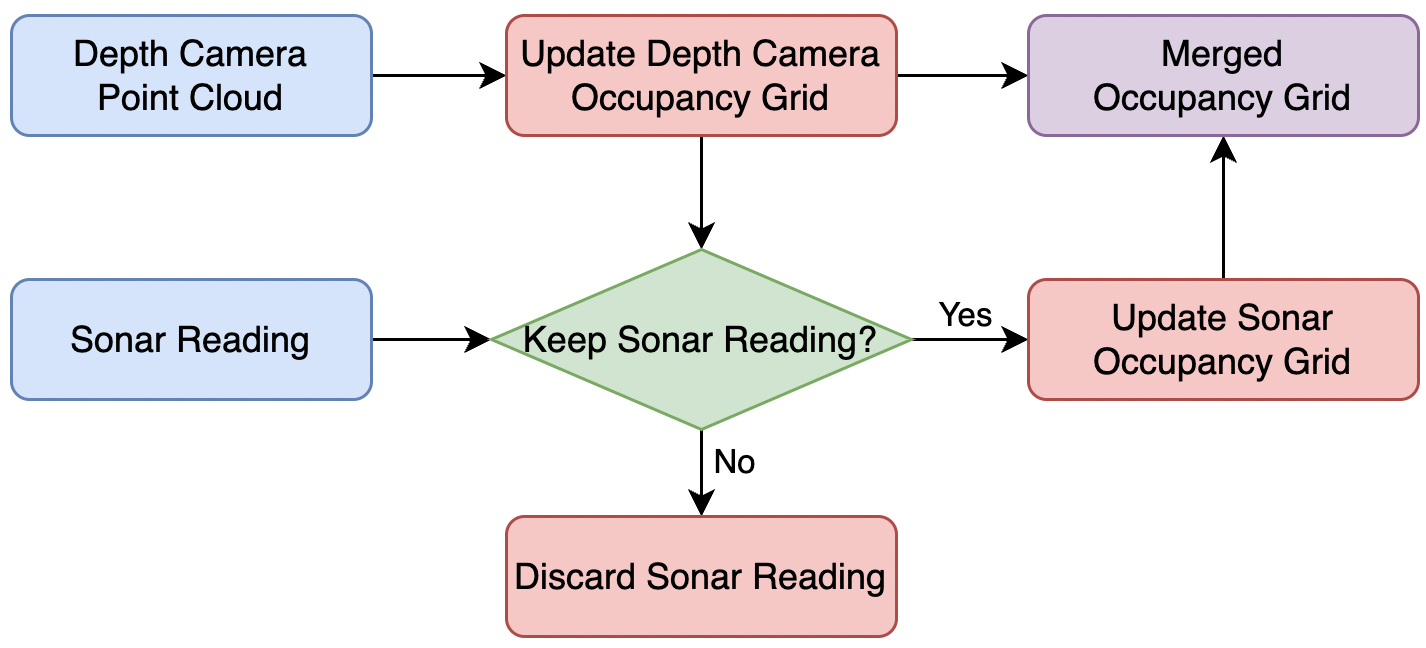
\includegraphics[width=0.8\columnwidth]{fig/occ_flow.png}
    \caption{Flow chart of occupancy map update.}
    \label{fig:occ_flow}
\end{figure}

To demonstrate the effectiveness of our approach, we compare the occupancy map built solely using depth images with the occupancy map maintained by fusing depth images and sonar readings in Fig. \ref{fig:occ_comp}. We observe that the depth-images-only map fails to mark the center region of the wall as occupied, which corresponds to a simulated glass window. In contrast, the merged map successfully marks the glass region as occupied based on sonar readings while retaining accurate information on the other parts of the environment provided by depth images.

\begin{figure}[h]
    \centering
    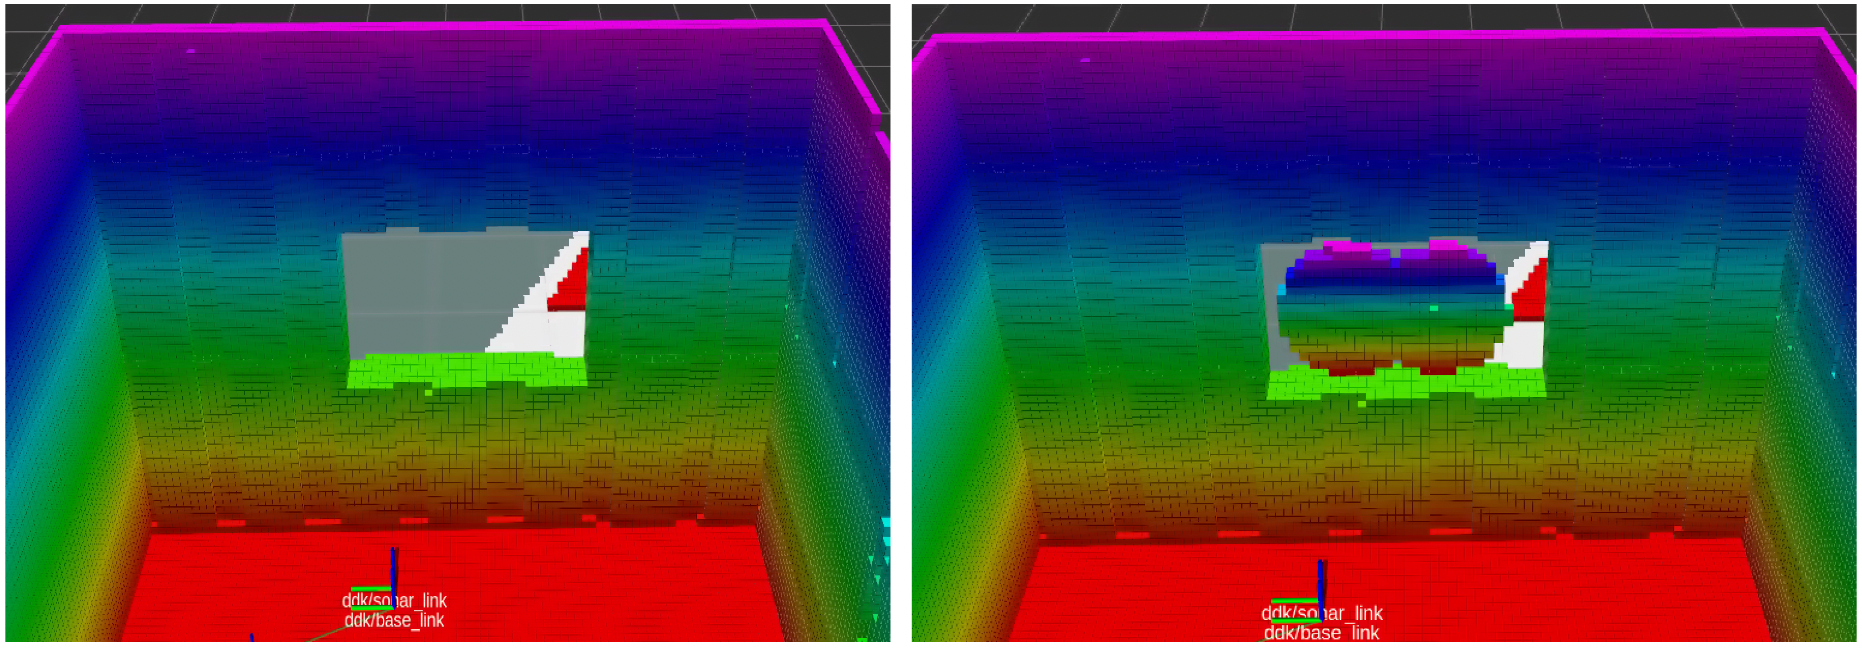
\includegraphics[width=1\columnwidth]{fig/occ_comp.png}
    \caption{Map built on depth images vs. sonar readings \& depth images.}
    \label{fig:occ_comp}
\end{figure}

\subsection{RANSAC-based Window Segmentation}
\label{sec:method_ransac}
In certain scenarios, particularly in indoor exploration, it is advantageous to have semantic knowledge about the location of windows. Such information may enhance the efficiency of exploration logistics. In this study, we propose a RANSAC-based approach for window segmentation. The method initially identifies the region of interest based on the discrepancy between the sonar reading and the depth-image-based occupancy map. Then, the potential location of the window is further determined by its geometric characteristics. The flowchart illustrated in Fig. \ref{fig:ransac_flow} depicts the mechanism.

\begin{figure}[h]
    \centering
    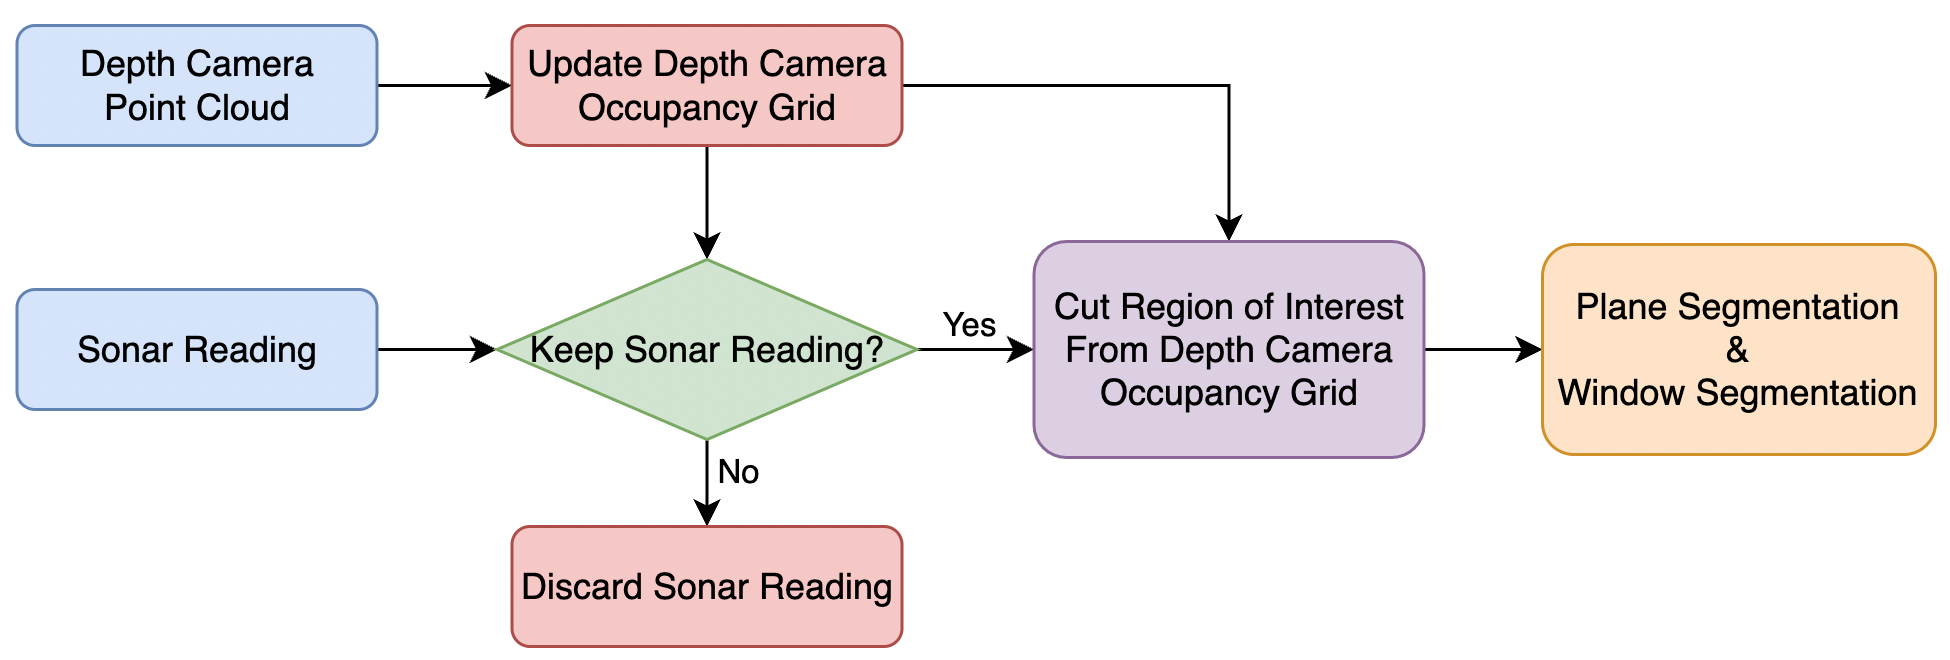
\includegraphics[width=1\columnwidth]{fig/ransac_flow.png}
    \caption{Flow chart of RANSAC-based Window Segmentation.}
    \label{fig:ransac_flow}
\end{figure}

As seen from Fig. \ref{fig:ransac_flow}, the segmentation process's initial stage is precisely the same as the occupancy map update pipeline. The sonar reading that contains valuable information is determined first. Since the sonar reading is retained only when it detects potential obstacles that are not detected by the depth camera, a window is likely to exist in the sonar reading's vicinity. Therefore, we consider the center point of the sonar reading (i.e., the center of the sonar beam's bottom surface) as the pivot and extract a region of interest in the size of a 5-meter by 5-meter box with a height of 3 meters.

Next, we utilize the SACSegmentation pipeline, which is supported by the PCL library, to segment the largest plane in the region of interest. If the magnitude of the $z$ coefficient of the fitted plane is below a certain threshold (e.g., 0.01), the plane is nearly vertical to the ground plane, which indicates that it is highly likely to represent a straight wall in an indoor environment. In the left-hand side of Fig. \ref{fig:ransac}, an example of fitted vertical planes can be seen. The white regions represent all inlier grid cells. However, due to simulated sensor noise, the occupancy representation of a flat wall may not appear completely flat. As a result, there may be several vertical gaps among white regions.

The final stage involves searching along the fitted plane for any rectangular openings, which represent the potential window region. The occupancy grid provides us with a discretized representation of the fitted plane, allowing us to search the plane vertically line by line. For each line, we count the number of unoccupied cells. Finally, we consider the region framed by vertical lines that contain a similar number of free-space cells as the potential glass region.

\begin{figure}[h]
    \centering
    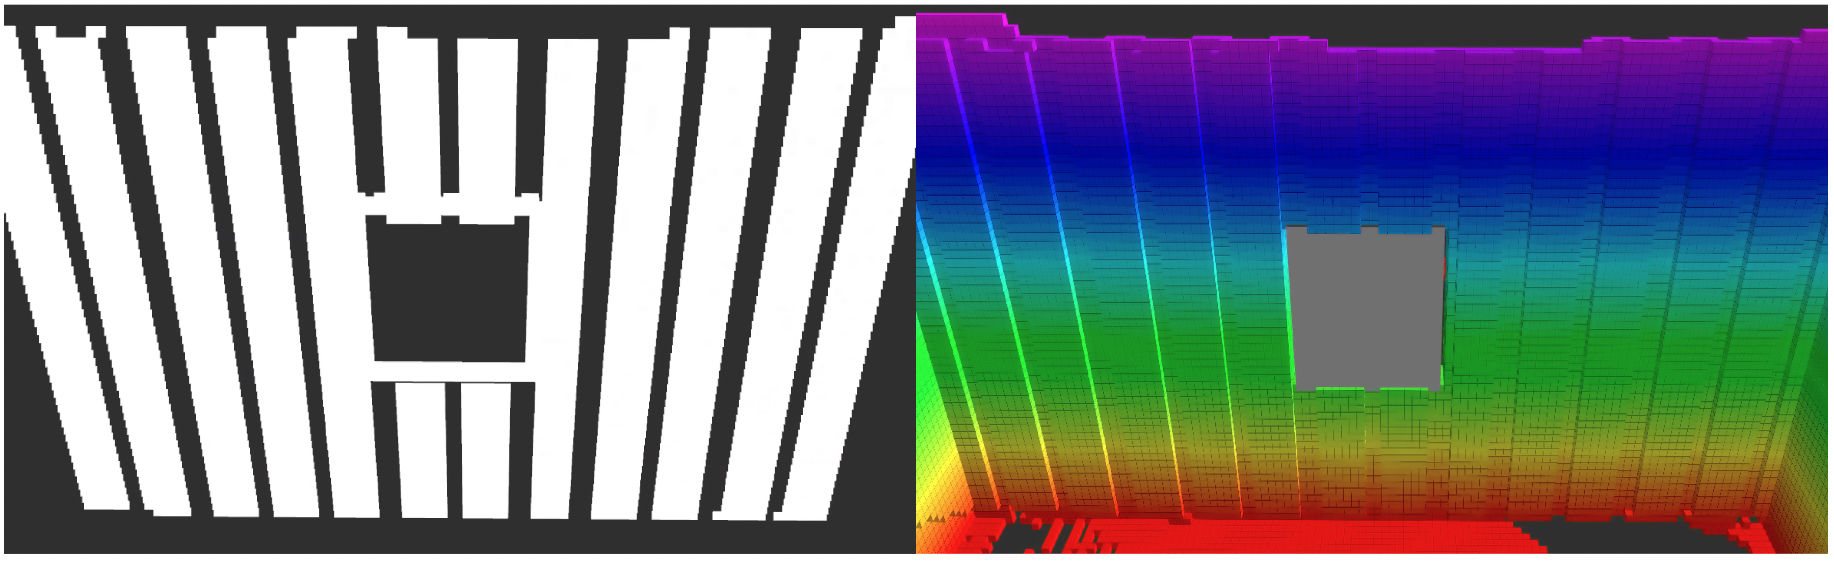
\includegraphics[width=1\columnwidth]{fig/ransac.png}
    \caption{RANSAC-based Window Detection. The left image displays all the inliers on the fitted largest plane. The right image depicts the occupancy map, with the window segmentation marked in grey.}
    \label{fig:ransac}
\end{figure}

The right-hand side of Fig. \ref{fig:ransac} shows an example of the segmented window area, which is marked in grey and framed by the colorful depth-camera-based occupancy grids.
    
    \section{Conclusion}
\label{sec:conclusion}
In conclusion, this study investigates the feasibility of integrating ultrasonic sensors as a secondary sensing modality to current mapping stacks in robotics. The study developed simulation environments, implemented sensor fusion mechanisms, and designed a RANSAC-based approach for window segmentation. The combination of depth cameras as the primary sensing device and sonar data as heuristic information can provide better safety and environmental understanding for robot navigation.

    \section{Discussion and Future Work}
\label{sec:discussion}

\subsection{Limitations}
Firstly, the sonar reading is determined useful only when almost all the grid cells within the sonar beam are marked as free space in the depth-camera-based occupancy map. However, due to the inherent inaccuracies and wide-angle nature of the actual sonar sensor (0.5 rad), this condition can only be satisfied when the drone is positioned very close to the window region and is facing directly at the main part of the window, rather than the window edge. Thus, detecting window regions using sonar requires the drone to be in very close proximity and to have a clear view of the window, limiting its usefulness in scenarios where the drone cannot get close enough or has obstructed views.

Secondly, the RANSAC-based plane segmentation technique may not be robust enough to handle real-life indoor settings where there are many obstacles such as tables, chairs, and other objects that can interfere with the segmentation process. This could result in incorrect segmentation and affect the accuracy of the final window detection.

Furthermore, the window segmentation approach assumes that the window is surrounded by solid, camera-visible walls, which may not always be the case in real-life scenarios. For example, some large windows may only have thin metal frames among the window patches, which could affect the segmentation process. Additionally, the approach may not be applicable to large tilted windows such as the one found in the PERCH meeting room. Therefore, while the proposed approach provides a good starting point, further research and development is needed to address these limitations and ensure its effectiveness in a wider range of scenarios.

\subsection{Future Work}
The current system faces certain bottleneck due to the limitations of the sonar hardware used, which provides only a scalar reading in the frequency around 8Hz. When compared to a typical depth camera that can provide a depth image of 720x480 or larger, the single sonar measurement is significantly limited and of low accuracy. In some prior work, researchers have utilized sonar arrays, with each sensor pointing at different angles. However, this approach is mostly limited to ground vehicles as it adds significant payload to a \gls{uav} platform. Although 3D sonar sensors, such as TOPOSENS 3D Ultrasonic Sensors introduced in \cite{Toposens2020}, provide image-like distance measurements, they are also heavy and power-consuming, making integration onto a \gls{uav} not feasible.

The polarization camera is an intriguing alternative sensor worth considering. When light reflects off a glass surface, it becomes partially polarized, meaning that the reflected light waves oscillate in a particular direction. A polarization camera is able to detect this polarization by measuring the orientation of the oscillation of the reflected light waves. This allows the camera to distinguish between glass surfaces and other materials that do not polarize light in the same way, such as walls or desks. There exists several work which use polarization cues for transparent object segmentation \cite{deeppolar} and glass segmentation \cite{glasspolar}. However, this field still holds great potential for further investigation. One possible direction for future research is to integrate the polarization camera onto the \gls{uav} platform and fuse the data provided by the polarization camera and RGB-D camera using learning-based approach. Doing so may create a more reliable mechanism for window segmentation, thus improving the safety of \gls{uav} navigation and providing valuable semantic information for exploration tasks.

% \newpage
\bibliography{literature}

\end{document}

